\documentclass[a4paper,10pt]{article}

%%%%%%%%%%%%%%%%%%%%%%%%%%%%%%%%%%%%%%%%

\usepackage{graphicx}
\usepackage[english]{babel}
\usepackage[latin1]{inputenc}
\usepackage{pgfplots}
\usepackage{hyperref}

\pgfplotsset{width=10cm,compat=1.9}

%%%%%%%%%%%%%%%%%%%%%%%%%%%%%%%%%%%%%%%%

\begin{document}

%%%%%%%%%%%%%%%%%%%%%%%%%%%%%%%%%%%%%%%%
% Frontpage

\title{Parallelizing HPCpp code}
\author{Agust\'in Mista\\ mista@chalmers.se}
\date{}
\maketitle

%%%%%%%%%%%%%%%%%%%%%%%%%%%%%%%%%%%%%%%%
% Sections

\section*{Introduction}

HPCpp \cite{hpcpp} is a fork of the Haskell Program Coverage tool (HPC)
\cite{hpc} that can process multiple coverage files at once, combining them to
produce fine-grain reports with detailed information about which property of the
test suite produced each tick in the code during testing.

In the future, I plan to extend the ideas behind HPCpp in two possible
directions: i) creating dynamic reports (inspired by QuickCheck-CI), and ii)
automated test suite reduction based on coverage.
%
However, for these ideas to work in practice, I need not only suitable
representation for the coverage information (that now comes from multiple
inputs), but also a basic set of fast operations to manipulate it.
%
This report explores the process of implementing and improving the performance
of such representation and operations using parallelism and playing with
different data structures.\footnote{All the code and results I present on this
  report can be found at
  \url{https://github.com/agustinmista/hpcpp/tree/master/bench}}.

\section*{Setup}

\paragraph{Case studies}
With the hope of having somewhat representative results, I picked three case
studies to be benchmarked in this report:

\begin{itemize}
\item \textbf{bst}: an implementation of binary search trees by John Hughes.
  Contains 79 individial coverage (tix) files adding up to 354kb of data.
\item \textbf{primitive}: the test suite of the package
  \texttt{packages-primitive}, which implements some of GHC's primitive
  memory-related operations \cite{primitive}. Contains 86 individual tix files
  adding up to 2.4Mb of data.
\item \textbf{xmonad}: the test suite of the package \texttt{xmonad}, which
  implements the popular windows manager for Linux \cite{xmonad}. Contains 119
  individual tix files adding up to 1.88Mb of data.
\end{itemize}

Each case study contains as many tix files as QuickCheck properties are defined
in their corresponding test suites.
%
They were generated after running each test suite using either a patched version
of \texttt{tasty-quickcheck} \cite{tasty-quickcheck-hpc} (\textbf{bst} and
\textbf{primitive}), or a manually patched test suite (\textbf{xmonad}).

\paragraph{Platform}
I used Criterion to implement every benchmark shown in this report.
%
More specifically, the times shown correspond to the mean ones reported by
Criterion.
%
To run them, I used a desktop machine with a 6 cores (12 threads) CPU (Intel(R)
Core(TM) i7-8700 CPU @ 3.20GHz) and 32gb of RAM.


The GHC version used to compile the code is 8.10.2, with the \texttt{-O2},
\texttt{-threaded} and \texttt{-feager-blackholing} flags.
%
As for the RTS flags, I set the stack, heap and nursery size to 200Mb
(\texttt{-K200m}, \texttt{-H200m}, and \texttt{-A200m}, respectively).
%
All the sequential implementations were benchmarked using a single core
(\texttt{-N1}), whereas the parallel ones were bencharked varying the number of
cores from 1 to 6.

\section*{Sequential implementation and variants}

In this section I briefly describe the sequential implementation of the code I
used as an initial baseline, along with two variants using different data
structures to store different parts the data.

The tix files generated by HPC use a simple representation: a list of tix
modules, where each tix module contains a list of coverage ticks (of type
\texttt{[Integer]}) and some metadata:

\begin{verbatim}
data Tix = Tix [TixModule]
data TixModule = TixModule String Hash Int [Integer]
\end{verbatim}

In my implementation, I want to be able to distinguish which property produced
each tick, so instead of using \texttt{Integer}s, I use a mapping from property
names to ticks (\texttt{TicksCount}), the rest of the data is simply a mirror
from that of the original tix implementation:

\begin{verbatim}
data MTix = MTix [MTixModule]
data MTixModule = MTixModule String Hash Int [TicksCount]
type TicksCount = [(String, Integer)]
\end{verbatim}

Using these data types, I am interested in four main operations: \textit{read},
\textit{merge}, \textit{project} and \textit{expression coverage}, which I
describe in detail below.

\paragraph{Reading}

The first operation takes care of reading and parsing the input tix files. For
this, I rely on the original HPC implementation (\texttt{readTix}), and wrap it
with a transformation from \texttt{Tix} to \texttt{MTix} that creates a
singleton tick count for each tick on the original tix file:

\begin{verbatim}
readMTixs :: [FilePath] -> IO [MTix]
readMTixs = mapM readMTix

readMTix :: FilePath -> IO MTix
readMTix file = do
  mtix <- readTix file
  case mtix of
    Nothing -> error $ "error reading tix file from: " ++ file
    Just a -> return (tixToMTix (takeBaseName file) a)

tixToMTix :: String -> Tix -> MTix
tixToMTix prop (Tix xs) =
  MTix (toMTixModule <$> xs)
  where
    toMTixModule (TixModule n h i ticks) =
      MTixModule n h i (tick prop <$> ticks)
\end{verbatim}

\paragraph{Merging}

The second operation I consider in this implementation takes care of merging the
singleton \texttt{MTix} values I read using \texttt{readMTixs} into a single
\texttt{MTix} that encompasses all the information.
%
For this, I can simply fold the inputs using a merging operation.
%
This operation zips the singleton tick information using monoid concatenation
\texttt{(<>)} across every module:

\begin{verbatim}
mergeMTixs :: [MTix] -> MTix
mergeMTixs [] = error "mergeMTixs: empty input"
mergeMTixs xs = foldr1 mergeMTix xs

mergeMTix :: MTix -> MTix -> MTix
mergeMTix (MTix ts1) (MTix ts2) =
  MTix (zipWith mergeMTixModule ts1 ts2)

mergeMTixModule :: MTixModule -> MTixModule -> MTixModule
mergeMTixModule (MTixModule n1 h1 i1 tks1) (MTixModule n2 h2 i2 tks2)
  | n1 == n2 && h1 == h2 && i1 == i2 =
      MTixModule n1 h1 i1 (zipWith (<>) tks1 tks2)
  | otherwise =
      error "mismatched modules!"
\end{verbatim}

\paragraph{Projection}

The next operation I implemented serves the purpose of projecting specifing
properties from an \texttt{MTix} value, which can come in handy when
implementing a test suite reduction algorithm in the future.
%
This operation takes a list of properties to project and simply filters them on
every tick count:

\begin{verbatim}
projectMTix :: [String] -> MTix -> MTix
projectMTix props (MTix ts) = MTix (projectMTixModule props <$> ts)

projectMTixModule :: [String] -> MTixModule -> MTixModule
projectMTixModule props (MTixModule n h i tks) =
  MTixModule n h i (projectTicksCount props <$> tks)

projectTicksCount :: [String] -> TicksCount -> TicksCount
projectTicksCount props = filter ((`elem` props) . fst)
\end{verbatim}

\paragraph{Expression coverage}

The last operation I consider here takes care of calculating simple code
coverage statistics.
%
For simplicity, I only care about expression coverage here, but the
implementation for the rest of the criteria (alternatives, top-level
definitions, boolean conditions, etc.) supported by HPC should be analogous.
%
This operation is a bit more involved than the rest, as the long list of ticks
contained in the original tix files represents several kinds of syntactic
elements in the code (corresponding to the different criteria mentioned above),
and here we only care about those that represent expressions.
%
To distinguish them, we need to use a secondary set of files produced by HPC,
known as \emph{mix} files.
%
These files contain the \emph{kind} of tick associated to each tick value within
a tix module.


Here I assume that these auxiliary files are already parsed and are given as an
input to our algorithm, using a mapping from module names to their corresponding
mix information.
%
Then, our algorithm looks up for those ticks that represent expressions in the
code, and transform each one them into a tuple \emph{(covered, total)} that can
be folded across different modules in order to calculate expression coverage
statistics in a per-module basis:

\begin{verbatim}
expCoverMTix :: [(String, Mix)] -> MTix -> [(String, Double)]
expCoverMTix mixs (MTix mods) = do
  expCoverMTixModule mixs <$> mods

expCoverMTixModule :: [(String, Mix)] -> MTixModule -> (String, Double)
expCoverMTixModule mixs (MTixModule name hash size tix) = do
  (name, (fromIntegral cov * 100) / fromIntegral tot)
  where
    (cov, tot) = foldr expCover (0,0) (zip mix tix)
    Just (Mix _ _ _ _ mix)  = lookup (takeFileName name) mixs
    mixName (Mix m _ _ _ _) = takeFileName m

expCover :: (MixEntry, TicksCount)
         -> (Integer, Integer) -> (Integer, Integer)
expCover ((_, ExpBox _), ticks) (cov, tot)
  | ticksTotal ticks > 0  = (cov+1, tot+1)
  | otherwise             = (cov,   tot+1)
expCover _ (cov, tot)     = (cov,   tot)
\end{verbatim}

\subsection*{Implementation variants}

The initial implementation uses lists everywhere, which are usually a concern
when it comes to performance.
%
For this reason, I decided to implement two different variants of the
implementation above, changing some data structures here and there:

\begin{itemize}
\item \textbf{SeqList}: the sequential implementation using lists shown above.
\item \textbf{SeqMap}: like \textbf{SeqList}, except that individual tick counts
  are implemented using finite maps (implemented using balanced binary trees
  \cite{data-map}), as:
\begin{verbatim}
type TicksCount = Map String Integer
\end{verbatim}
\item \textbf{SeqSeq}: like \textbf{SeqMap}, except that modules use sequences
  of tick counts (implemented via 2-3 trees \cite{data-sequence}) instead of lists:
\begin{verbatim}
data MTixModule = MTixModule String Hash Int (Seq TicksCount)
\end{verbatim}
\end{itemize}

To compare these variants, I first ran each operation on each case study,
varying the input size from one to the full set of inputs.
%
The results there shown that the execution time \emph{always grows linearly over
  the number of inputs}, so I decided to only consider from now on: the full set
of inputs for the read, merge, and expression coverage operations, and half of
the inputs for the projection operation (so I do not end up with the same input
value as output).
%
With these considerations, the times required to perform each operation are as
shown below:\\

% Sequential times
\resizebox{\textwidth}{!}{
\hspace{-30pt}
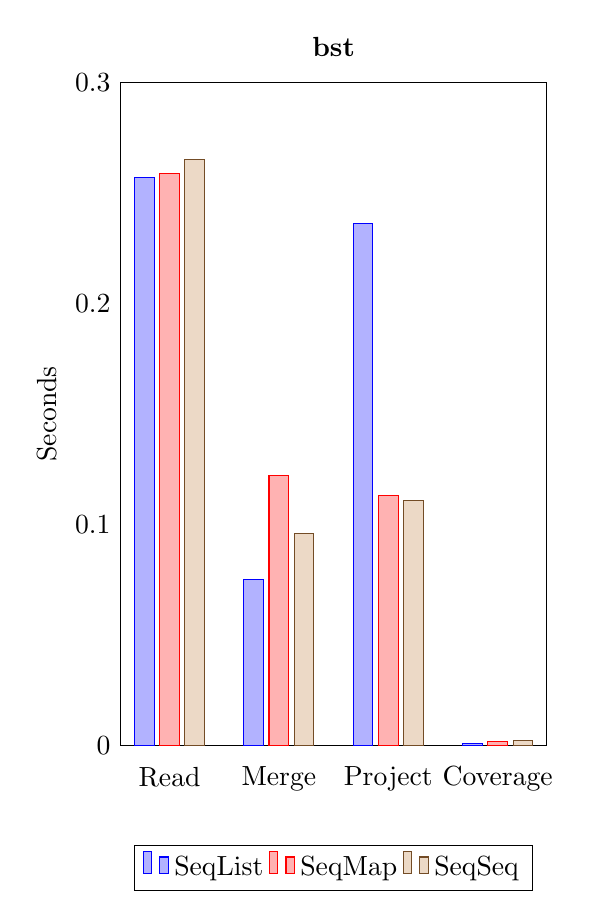
\begin{tikzpicture}
  \pgfplotsset{xtick style={draw=none}}
  \pgfplotsset{ytick style={draw=none}}
  \begin{axis}[
      bar width=0.25cm,
      width=7cm,
      height=10cm,
      ybar,
      enlargelimits=0.15,
      legend style={
        at={(0.5,-0.15)},
        anchor=north,legend columns=-1
      },
      enlarge y limits=0,
      ymax=0.3,
      ymin=0,
      ytick distance=0.1,
      xtick=data,
      title={\textbf{bst}},
      ylabel={Seconds},
      symbolic x coords={Read, Merge, Project, Coverage},
    ]
    \addplot coordinates {(Read,0.257) (Merge,0.075) (Project,0.236) (Coverage, 0.0007)};
    \addplot coordinates {(Read,0.259) (Merge,0.122) (Project,0.113) (Coverage, 0.0018)};
    \addplot coordinates {(Read,0.265) (Merge,0.096) (Project,0.111) (Coverage, 0.0020)};
    \legend{SeqList, SeqMap, SeqSeq}
  \end{axis}
\end{tikzpicture}
~\hspace{-15pt}
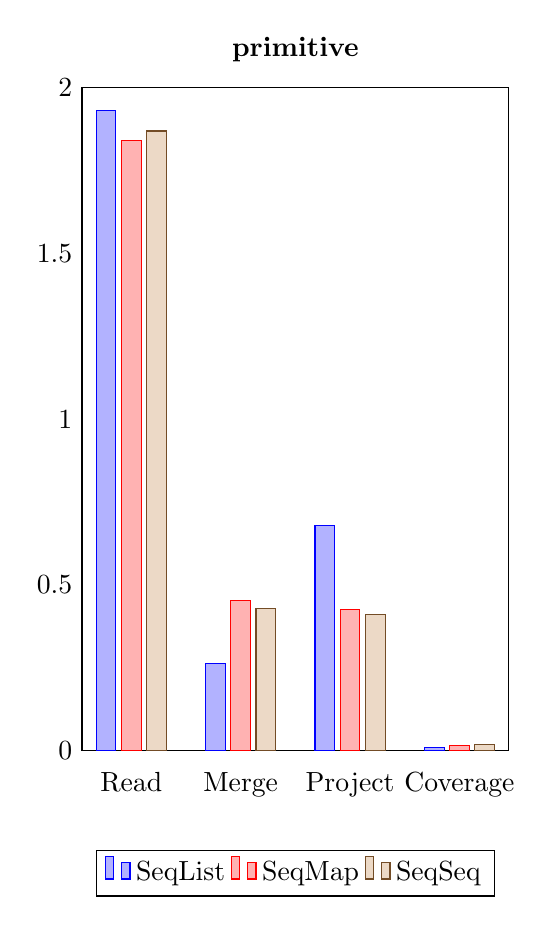
\begin{tikzpicture}
  \pgfplotsset{xtick style={draw=none}}
  \pgfplotsset{ytick style={draw=none}}
  \begin{axis}[
      bar width=0.25cm,
      width=7cm,
      height=10cm,
      ybar,
      enlargelimits=0.15,
      legend style={
        at={(0.5,-0.15)},
        anchor=north,legend columns=-1
      },
      enlarge y limits=0,
      ymax=2,
      ymin=0,
      ytick distance=0.5,
      xtick=data,
      title={\textbf{primitive}},
      symbolic x coords={Read, Merge, Project, Coverage},
    ]
    \addplot coordinates {(Read,1.931) (Merge,0.262) (Project,0.680) (Coverage, 0.010)};
    \addplot coordinates {(Read,1.841) (Merge,0.452) (Project,0.426) (Coverage, 0.015)};
    \addplot coordinates {(Read,1.870) (Merge,0.429) (Project,0.412) (Coverage, 0.018)};
    \legend{SeqList, SeqMap, SeqSeq}
  \end{axis}
\end{tikzpicture}
~\hspace{-15pt}
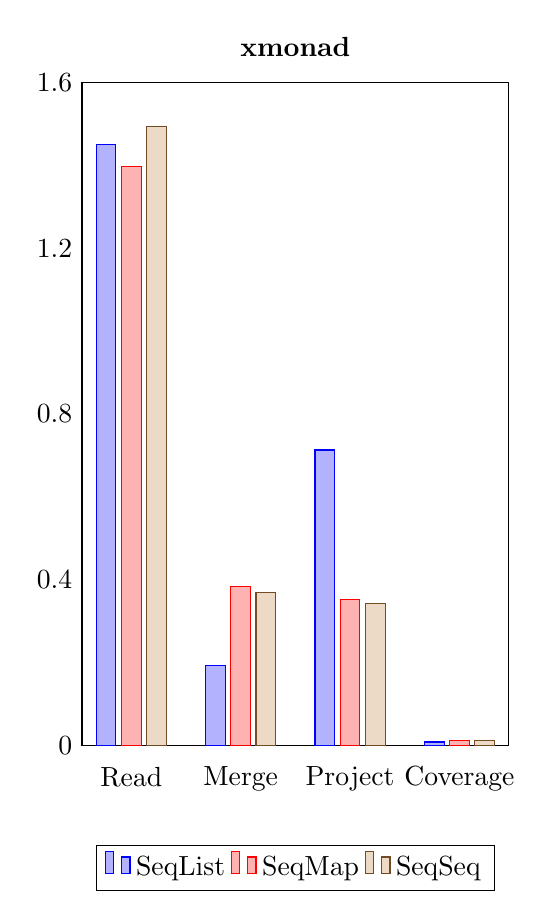
\begin{tikzpicture}
  \pgfplotsset{xtick style={draw=none}}
  \pgfplotsset{ytick style={draw=none}}
  \begin{axis}[
      bar width=0.25cm,
      width=7cm,
      height=10cm,
      ybar,
      enlargelimits=0.15,
      legend style={
        at={(0.5,-0.15)},
        anchor=north,legend columns=-1
      },
      enlarge y limits=0,
      ymax=1.6,
      ymin=0,
      ytick distance=0.4,
      xtick=data,
      title={\textbf{xmonad}},
      symbolic x coords={Read, Merge, Project, Coverage},
    ]
    \addplot coordinates {(Read,1.450) (Merge,0.193) (Project,0.713) (Coverage, 0.008)};
    \addplot coordinates {(Read,1.398) (Merge,0.383) (Project,0.353) (Coverage, 0.011)};
    \addplot coordinates {(Read,1.493) (Merge,0.368) (Project,0.343) (Coverage, 0.012)};
    \legend{SeqList, SeqMap, SeqSeq}
  \end{axis}
\end{tikzpicture}
}\\

And since the expression coverage operation takes a considerably shorter time on
average, below is a ``zoomed'' version of the times required by this operation
(notice the Y scale is in milliseconds!):\\

% Zoomed coverage
\resizebox{0.4\textwidth}{!}{
\hspace{-20pt}
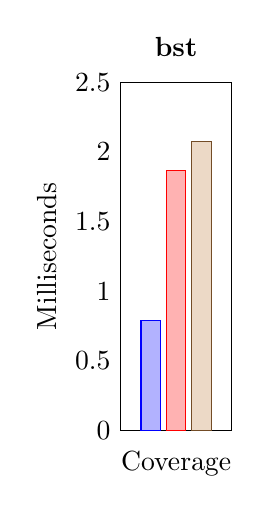
\begin{tikzpicture}
  \pgfplotsset{xtick style={draw=none}}
  \pgfplotsset{ytick style={draw=none}}
  \begin{axis}[
      bar width=0.25cm,
      width=3cm,
      height=6cm,
      ybar,
      enlargelimits=0.15,
      enlarge y limits=0,
      ymax=2.5,
      ymin=0,
      ytick distance=0.5,
      xtick=data,
      ylabel={Milliseconds},
      title={\textbf{bst}},
      symbolic x coords={Read, Merge, Project, Coverage},
    ]
    \addplot coordinates {(Coverage, 0.791)};
    \addplot coordinates {(Coverage, 1.870)};
    \addplot coordinates {(Coverage, 2.076)};
    \legend{}
  \end{axis}
\end{tikzpicture}
~\hspace{-5pt}
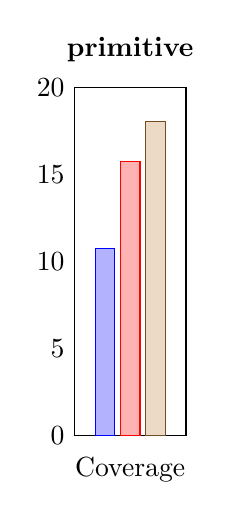
\begin{tikzpicture}
  \pgfplotsset{xtick style={draw=none}}
  \pgfplotsset{ytick style={draw=none}}
  \begin{axis}[
      bar width=0.25cm,
      width=3cm,
      height=6cm,
      ybar,
      enlargelimits=0.15,
      enlarge y limits=0,
      ymax=20,
      ymin=0,
      ytick distance=5,
      xtick=data,
      title={\textbf{primitive}},
      symbolic x coords={Read, Merge, Project, Coverage},
    ]
    \addplot coordinates {(Coverage, 10.78)};
    \addplot coordinates {(Coverage, 15.77)};
    \addplot coordinates {(Coverage, 18.09)};
    \legend{}
  \end{axis}
\end{tikzpicture}
~\hspace{-5pt}
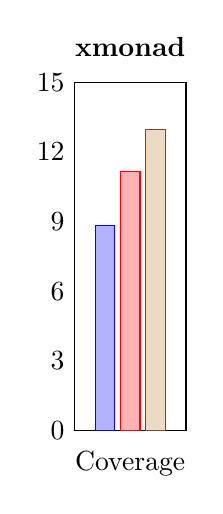
\begin{tikzpicture}
  \pgfplotsset{xtick style={draw=none}}
  \pgfplotsset{ytick style={draw=none}}
  \begin{axis}[
      bar width=0.25cm,
      width=3cm,
      height=6cm,
      ybar,
      enlargelimits=0.15,
      enlarge y limits=0,
      ymax=15,
      ymin=0,
      ytick distance=3,
      xtick=data,
      title={\textbf{xmonad}},
      symbolic x coords={Read, Merge, Project, Coverage},
    ]
    \addplot coordinates {(Coverage, 8.843)};
    \addplot coordinates {(Coverage, 11.150)};
    \addplot coordinates {(Coverage, 12.986)};
    \legend{}
  \end{axis}
\end{tikzpicture}
}

At simple sight, it seems that the larger improvement comes from using finite
maps for tick counts when performing projections.
%
The rest of the operations show some slowdown when using data structures other
than lists, due to better deforestation support and optimization rules for lists
perhaps?
%
Using sequences slightly helps reducing times when merging, and projecting, but
adds a little overhead when reading and measuring coverage.

After these observations, I decided to continue the benchmarks using the
\textbf{SeqSeq} variant as the baseline for the sequential implementation when
comparing with other parallel ones (implemented as variants of \textbf{SeqSeq}).


\section*{Parallel implementations}

It is finally time to start speeding things up using more than one CPU core at a
time.
%
In this section I present different parallel variants of each of the four
operations described so far.

An important thing to notice is that all the parallel variants I present in this
section are implemented using parallel strategies from the \texttt{parallel}
package \cite{seq-no-more} by Simon Marlow.
%
I did not find noticeable differences when trying to implement them using the
\texttt{Par} monad, so I saw no point in comparing them here.


\subsection*{Parallel Read}

To parallelize this operation I simply make sure that each element of the output
is evaluated in parallel on a different spark:

\begin{verbatim}
readMTixs :: [FilePath] -> IO [MTix]
readMTixs files = do
  mtixs <- mapM readMTix files
  return (mtixs `using` parList rdeepseq)
\end{verbatim}

Acording to ThreadScope, this simple tweak produces a nice green block of CPU
usage when ran in parallel using 6 cores for the \textbf{primitive} case study
(the rest of the ThreadScope figures on this report were obtained using the same
case study and number of cores):\\

\begin{center}
  \includegraphics[scale=0.3]{threadscope/ParRead}
\end{center}

I suspect that the single threaded work that happens at the beginning of this
operation could be a consequence of listing the directory where inputs are
located using the \texttt{System.Directory.listDirectory} function.

\paragraph{Benchmarks}
I benchmarked this operation in function of the number of CPU cores used on each
case study:\\

% Parallel read
\resizebox{\textwidth}{!}{
\hspace{-50pt}
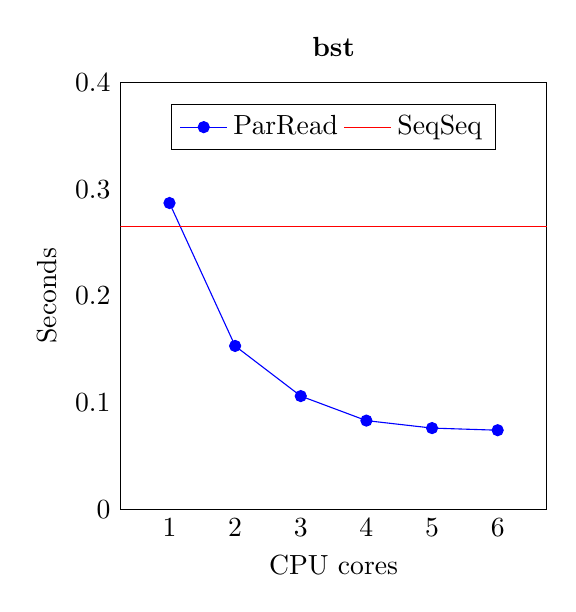
\begin{tikzpicture}
  \pgfplotsset{xtick style={draw=none}}
  \pgfplotsset{ytick style={draw=none}}
  \begin{axis}[
      width=7cm,
      height=7cm,
      enlargelimits=0.15,
      enlarge y limits=0,
      ymax=0.4,
      ymin=0,
      ytick distance=0.1,
      xtick=data,
      ylabel={Seconds},
      xlabel={CPU cores},
      xmin=1,
      xmax=6,
      xtick distance=1,
      title={\textbf{bst}},
      legend style={
        at={(0.5,0.95)},
        anchor=north,legend columns=-1
      }
    ]
    \addplot[mark=*, blue] coordinates {
      (1, 0.287)
      (2, 0.153)
      (3, 0.106)
      (4, 0.083)
      (5, 0.076)
      (6, 0.074)
    };
    \addplot[mark=none, red] coordinates {
      (0,0.265) (7,0.265)
    };
    \legend{ParRead, SeqSeq}
  \end{axis}
\end{tikzpicture}
~\hspace{-5pt}
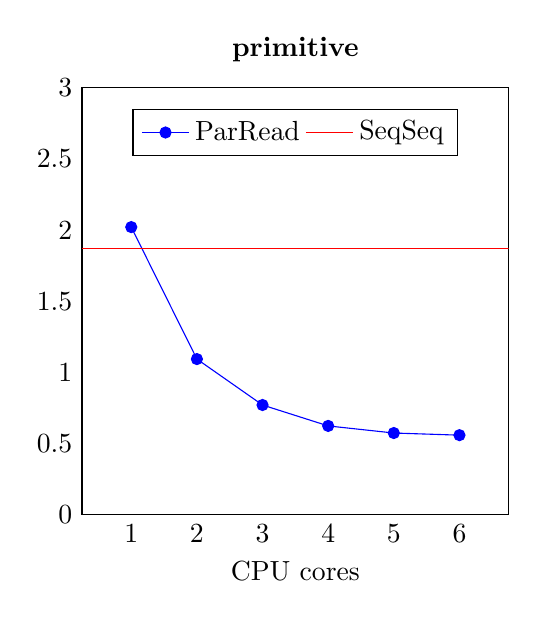
\begin{tikzpicture}
  \pgfplotsset{xtick style={draw=none}}
  \pgfplotsset{ytick style={draw=none}}
  \begin{axis}[
      width=7cm,
      height=7cm,
      enlargelimits=0.15,
      enlarge y limits=0,
      ymax=3,
      ymin=0,
      ytick distance=0.5,
      xtick=data,
      xlabel={CPU cores},
      xmin=1,
      xmax=6,
      xtick distance=1,
      title={\textbf{primitive}},
      legend style={
        at={(0.5,0.95)},
        anchor=north,legend columns=-1
      }
    ]
    \addplot[mark=*, blue] coordinates {
      (1, 2.021)
      (2, 1.093)
      (3, 0.770)
      (4, 0.623)
      (5, 0.573)
      (6, 0.558)
    };
    \addplot[mark=none, red] coordinates {
      (0,1.870) (7,1.870)
    };
    \legend{ParRead, SeqSeq}
  \end{axis}
\end{tikzpicture}
~\hspace{-5pt}
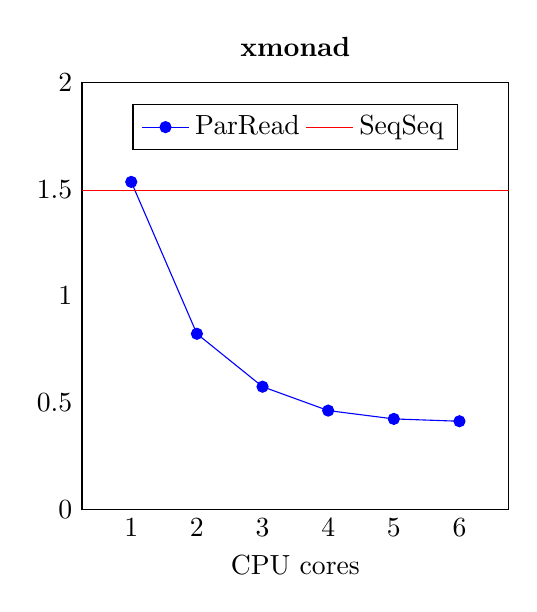
\begin{tikzpicture}
  \pgfplotsset{xtick style={draw=none}}
  \pgfplotsset{ytick style={draw=none}}
  \begin{axis}[
      width=7cm,
      height=7cm,
      enlargelimits=0.15,
      enlarge y limits=0,
      ymax=2,
      ymin=0,
      ytick distance=0.5,
      xtick=data,
      xlabel={CPU cores},
      xmin=1,
      xmax=6,
      xtick distance=1,
      title={\textbf{xmonad}},
      legend style={
        at={(0.5,0.95)},
        anchor=north,legend columns=-1
      }
    ]
    \addplot[mark=*, blue] coordinates {
      (1, 1.534)
      (2, 0.822)
      (3, 0.574)
      (4, 0.462)
      (5, 0.423)
      (6, 0.412)
    };
    \addplot[mark=none, red] coordinates {
      (0,1.493) (7,1.493)
    };
    \legend{ParRead, SeqSeq}
  \end{axis}
\end{tikzpicture}
}\\

These results indicate that it is possible to obtain a performance increase of
around 3.5x when using 6 CPU cores.
%
With this result in place, I decided to move onto the next operation, since
obtaining an ideal $\sim$6x speedup will be very unlikely to happen due to
the added overhead.
%
Also, I consider than spliting the input in a very small number of chunks will
hardly make things better, as we only have a handful of inputs (a couple of
hundreds at most), which should not incur into a noticeable overhead in terms of
sparked computations.
%
By the contrary, it could harm the performance if some chunk contains inputs
larger than the average.

\subsection*{Parallel Merge}

Parallelizing this operation was quite problematic, as every parallel
implementation I tried ended up being much slower than the sequential one.
%
After dozens of combinations of implementations, evaluation strategies,
compilation flags, RTS flags, parallel frameworks, I could not find a single one
that could show a noticeable speedup versus the sequential baseline.
%
By the contrary, none of them seemed to be able to be even on par to the
baseline.

At the light of these sad results, I decided to carry on and report three
implementations using different parallel granularity and analyse what could be
happening.

\paragraph{ParMerge1}

In this first implementation, I decided to parallelize the \texttt{mergeMTix}
operation using a bottom-up reduction approach, exploiting the associativity of
this binary operation:

\begin{verbatim}
mergeMTixs :: [MTix] -> MTix
mergeMTixs [] = error "mergeMTixs: empty input"
mergeMTixs xs = parFold1 rdeepseq mergeMTix xs

parFold1 :: Strategy a -> (a -> a -> a) -> [a] -> a
parFold1 s f [x] = x
parFold1 s f xs = parFold1 s f (reduce1 f xs `using` parList s)
\end{verbatim}

\begin{verbatim}
reduce1 :: (a -> a -> a) -> [a] -> [a]
reduce1 _ [] = []
reduce1 _ [x] = [x]
reduce1 f (x:y:ys) = f x y : reduce1 f ys
\end{verbatim}

Inspecting the ThreadScope output, we can see that some parallelism is happening
during the computation:\\

\includegraphics[scale=0.3]{threadscope/ParMerge1}\\

The shape of the CPU activity is easy to interpret: the first levels in the
bottom-up reduction strategy contain at least a few pairs of inputs that can be
sparked in parallel.
%
However, as we approach the last levels, we only have a handful of pairs of
larger values to merge, thus some CPUs will eventually start idling.
%
In the last level, we only have two very large values to merge, and this
operation will be sparked in a single CPU, taking most of the computation time.

In principle, this result would suggest that we have the wrong parallel
granularity in this implementation, though it should not be much slower than
the sequential version.

\paragraph{ParMerge2}

In the second variant of this operation, I moved the paralelism to the module
level, processing the fold operation sequentially, and zipping
\texttt{MTixModule}s in parallel via a parallel version of the \texttt{zipWith}
combinator:

\begin{verbatim}
mergeMTixs :: [MTix] -> MTix
mergeMTixs [] = error "mergeMTixs: empty input"
mergeMTixs xs = foldr1 mergeMTix xs

mergeMTix :: MTix -> MTix -> MTix
mergeMTix (MTix ts1) (MTix ts2) =
  MTix (parZipWith rdeepseq mergeMTixModule ts1 ts2)

parZipWith :: Strategy a -> (a -> a -> a) -> [a] -> [a] -> [a]
parZipWith s f xs ys = zipWith f xs ys `using` parList s
\end{verbatim}

This resulted in better CPU usage acording to ThreadScope, altought we can still
see a tail of uneven work:\\

\includegraphics[scale=0.3]{threadscope/ParMerge2}\\

However, this implementation is much slower than the previous unbalanced one!
(Benchmark results are at the end of this subsection.)

\paragraph{ParMerge3}

In a final attempt to parallelize this operation, I reduced the granularity to
chunks of tick entries on each module.
%
This is done similarly as before, except that I explicitly split the sequences
of tick entries of each module into the number of CPUs available, with a minimum
of 500 elements to ensure a reasonably large task on each spark:

\begin{verbatim}
mergeMTixs :: [MTix] -> MTix
mergeMTixs [] = error "mergeMTixs: empty input"
mergeMTixs xs = foldr1 mergeMTix xs

mergeMTix :: MTix -> MTix -> MTix
mergeMTix (MTix ts1) (MTix ts2) =
  MTix (parZipWith rdeepseq mergeMTixModule ts1 ts2)

mergeMTixModule :: MTixModule -> MTixModule -> MTixModule
mergeMTixModule (MTixModule n1 h1 i1 tks1) (MTixModule n2 h2 i2 tks2)
  | n1 == n2 && h1 == h2 && i1 == i2 =
      let n = max 500 (i1 `div` numCapabilities)
      in  MTixModule n1 h1 i1 (parSeqZipWithChunk rdeepseq n (<>) tks1 tks2)
  | otherwise =
      error "mismatched modules!"

parZipWith :: Strategy a -> (a -> a -> a) -> [a] -> [a] -> [a]
parZipWith s f xs ys = zipWith f xs ys `using` parList s

parSeqZipWithChunk :: Strategy (Seq a) -> Int -> (a -> a -> a)
                   -> Seq a -> Seq a -> Seq a
parSeqZipWithChunk s n f xs ys =
  concatSeqs (fmap zipChunk chunks `using` parTraversable s)
  where
    concatSeqs = foldr (Seq.><) Seq.empty
    zipChunk = fmap (\(x, y) -> f x y)
    chunks = Seq.chunksOf n (Seq.zip xs ys)
\end{verbatim}

The ThreadScope output for this implementation shows a similar result as before,
with a (slightly smaller) tail of uneven work:\\

\includegraphics[scale=0.3]{threadscope/ParMerge3}\\

More bad news, however. This implementation is even slower than the previous
one!
%
Also, given that the tail of uneven work has not dissapeared completely, I doubt
that the one on the previous implementation was caused due to a too coarse
granularity.

\paragraph{Benchmarks}

The benchmarks of the different variants I implemented for this operation show a
strange pattern: it seems that adding more CPU cores to the formula helps making
them faster, but the whole result is almost an order of magnitude slower:\\

% Parallel merge
\resizebox{\textwidth}{!}{
\hspace{-50pt}
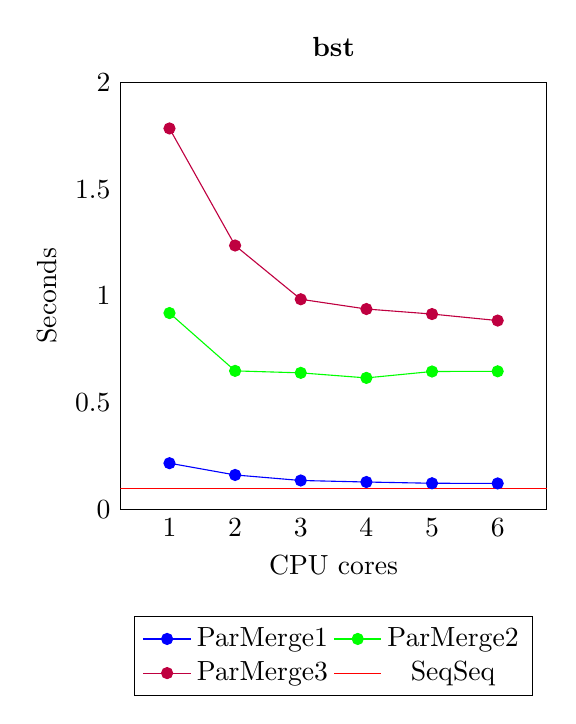
\begin{tikzpicture}
  \pgfplotsset{xtick style={draw=none}}
  \pgfplotsset{ytick style={draw=none}}
  \begin{axis}[
      width=7cm,
      height=7cm,
      enlargelimits=0.15,
      enlarge y limits=0,
      ymax=2,
      ymin=0,
      ytick distance=0.5,
      xtick=data,
      ylabel={Seconds},
      xlabel={CPU cores},
      xmin=1,
      xmax=6,
      xtick distance=1,
      title={\textbf{bst}},
      legend style={
        at={(0.5,-0.25)},
        anchor=north,legend columns=2
      }
    ]
    \addplot[mark=*, blue] coordinates {
      (1,	0.21536)
      (2,	0.16023)
      (3,	0.13433)
      (4,	0.12713)
      (5,	0.12131)
      (6,	0.12062)
    };
    \addplot[mark=*, green] coordinates {
      (1,	0.91919)
      (2,	0.64815)
      (3,	0.63881)
      (4,	0.61521)
      (5,	0.64522)
      (6,	0.64611)
    };
    \addplot[mark=*, purple] coordinates {
      (1,	1.78458)
      (2,	1.23577)
      (3,	0.98382)
      (4,	0.93810)
      (5,	0.91451)
      (6,	0.88399)
    };
    \addplot[mark=none, red] coordinates {
      (0,0.096)
      (7,0.096)
    };
    \legend{ParMerge1, ParMerge2, ParMerge3, SeqSeq}
  \end{axis}
\end{tikzpicture}
~\hspace{-5pt}
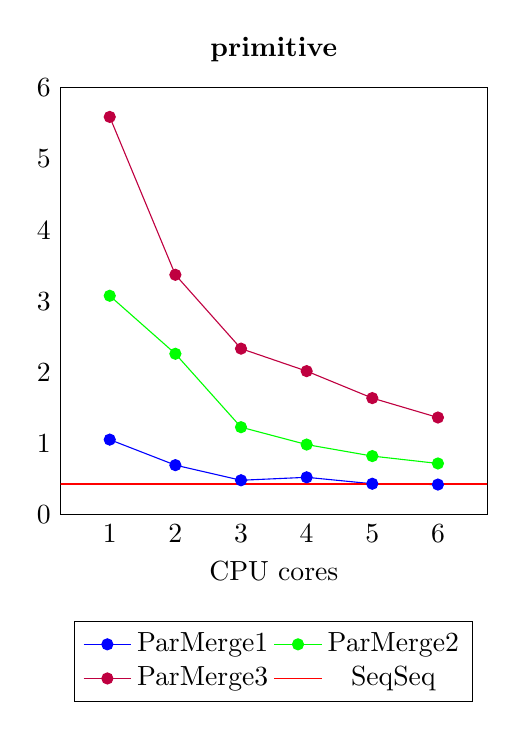
\begin{tikzpicture}
  \pgfplotsset{xtick style={draw=none}}
  \pgfplotsset{ytick style={draw=none}}
  \begin{axis}[
      width=7cm,
      height=7cm,
      enlargelimits=0.15,
      enlarge y limits=0,
      ymax=6,
      ymin=0,
      ytick distance=1,
      xtick=data,
      xlabel={CPU cores},
      xmin=1,
      xmax=6,
      xtick distance=1,
      title={\textbf{primitive}},
      legend style={
        at={(0.5,-0.25)},
        anchor=north,legend columns=2
      }
    ]
    \addplot[mark=*, blue] coordinates {
      (1,	1.05326)
      (2,	0.69427)
      (3,	0.48173)
      (4,	0.52334)
      (5,	0.43274)
      (6,	0.42144)
    };
    \addplot[mark=*, green] coordinates {
      (1,	3.07639)
      (2,	2.26061)
      (3,	1.22804)
      (4,	0.98374)
      (5,	0.82185)
      (6,	0.71797)
    };
    \addplot[mark=*, purple] coordinates {
      (1,	5.59171)
      (2,	3.37113)
      (3,	2.33293)
      (4,	2.01662)
      (5,	1.63729)
      (6,	1.36420)
    };
    \addplot[mark=none, red] coordinates {
      (0,0.429)
      (7,0.429)
    };
    \legend{ParMerge1, ParMerge2, ParMerge3, SeqSeq}
  \end{axis}
\end{tikzpicture}
~\hspace{-5pt}
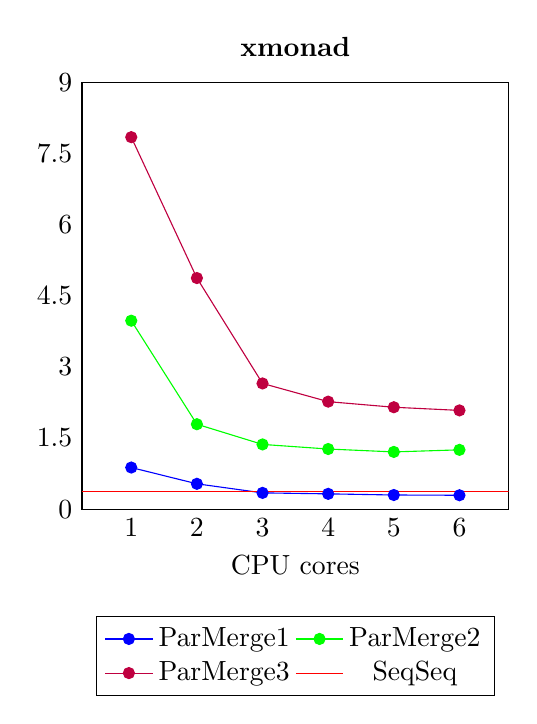
\begin{tikzpicture}
  \pgfplotsset{xtick style={draw=none}}
  \pgfplotsset{ytick style={draw=none}}
  \begin{axis}[
      width=7cm,
      height=7cm,
      enlargelimits=0.15,
      enlarge y limits=0,
      ymax=9,
      ymin=0,
      ytick distance=1.5,
      xtick=data,
      xlabel={CPU cores},
      xmin=1,
      xmax=6,
      xtick distance=1,
      title={\textbf{xmonad}},
      legend style={
        at={(0.5,-0.25)},
        anchor=north,legend columns=2
      }
    ]
    \addplot[mark=*, blue] coordinates {
      (1,	0.87770)
      (2,	0.53411)
      (3,	0.34285)
      (4,	0.32238)
      (5,	0.29815)
      (6,	0.29287)
    };
    \addplot[mark=*, green] coordinates {
      (1,	3.97514)
      (2,	1.79136)
      (3,	1.36511)
      (4,	1.26820)
      (5,	1.20695)
      (6,	1.25081)
    };
    \addplot[mark=*, purple] coordinates {
      (1,	7.84677)
      (2,	4.87466)
      (3,	2.65140)
      (4,	2.26753)
      (5,	2.14944)
      (6,	2.08265)
    };
    \addplot[mark=none, red] coordinates {
      (0,0.368)
      (7,0.368)
    };
    \legend{ParMerge1, ParMerge2, ParMerge3, SeqSeq}
  \end{axis}
\end{tikzpicture}
}\\

We can also notice that as we reduce the granularity of the parallel tasks, the
performance degrades considerably.
%
This effect would be reasonable if our code is spawning too many small parallel
sparks which contribute to the overhead.
%
However, the faster parallel implementation, \textbf{ParMerge1}, is the one that
clearly seemed it could benefit from a finer task granularity.

The reason behind the huge slowdowns of every implementation I tried remains a
mistery for me to this very day.
%
My best guess at what it going on is that the parallel evaluation strategy is
too strict, reducing subterms to normal form repeatedly. However, replacing
\texttt{rdeepseq} with different strategies resulted in computations that seem
to be running in a single core according to ThreadScope (no parallelism
whatsoever).
%
Another reason could be perhaps that the benchmark itself is for some reason
adding up the time required to reduce the output to normal form.
%
Hopefully, a reader trained in the art of parallelizing Haskell code will point
out what I did wrong.



\subsection*{Parallel Projection}

For the third operation, I implemented two variants of the projection operation,
which differ on the parallel task granularity.

\paragraph{ParProject1}

For this first attempt, I replaced the sequential map of
\texttt{projectMTixModule props} for its parallel counterpart, provided by the
\texttt{parallel} package:

\begin{verbatim}
projectMTix :: [String] -> MTix -> MTix
projectMTix props (MTix ts) =
  MTix (parMap rdeepseq (projectMTixModule props) ts)
\end{verbatim}

This simple solution produced a good amount of parallel CPU usage when inspected
using ThreadScope:\\

\includegraphics[scale=0.3]{threadscope/ParProject1}\\

Although I was not very happy about the tail of uneven parallel work at the end
of the computation, which was the motivation for reducing the task granularity
in the second variant.

\paragraph{ParProject2}

This variant works just like \textbf{ParProject1}, except that it also divides
the sequence of tick entries on each module in chunks that are processed in
parallel:

\begin{verbatim}
projectMTix :: [String] -> MTix -> MTix
projectMTix props (MTix ts) =
  MTix (parMap rdeepseq (projectMTixModule props) ts)

projectMTixModule :: [String] -> MTixModule -> MTixModule
projectMTixModule props (MTixModule n h i tks) =
  MTixModule n h i (parSeqMapChunk rdeepseq 50 (projectTicksCount props) tks)

parSeqMapChunk :: Strategy (Seq b) -> Int -> (a -> b) -> Seq a -> Seq b
parSeqMapChunk s n f xs =
  concatSeqs (fmap (fmap f) chunks `using` parTraversable s)
  where
    concatSeqs = foldr (Seq.><) Seq.empty
    chunks = Seq.chunksOf n xs
\end{verbatim}

The function \texttt{parSeqMapChunk} divides a sequence into chunks, evaluates
them in parallel, to finally concatenate them.
%
After manually tunning the chunk size, I found that processing chunks of 50
elements works well in most cases.

The ThreadScope output for this variant is as below:\\

\includegraphics[scale=0.3]{threadscope/ParProject2}\\

This result shows that this parallel computation now distributes work more
evenly across cores during its whole lifetime.

\paragraph{Benchmarks}
The benchmarks of both variants in terms of number of cores for each case study
are as shown below:\\

% Parallel project
\resizebox{\textwidth}{!}{
\hspace{-50pt}
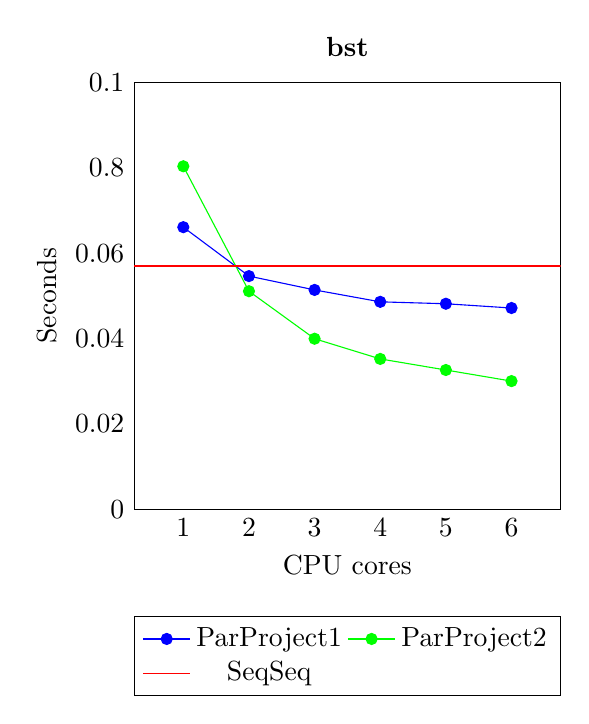
\begin{tikzpicture}
  \pgfplotsset{xtick style={draw=none}}
  \pgfplotsset{ytick style={draw=none}}
  \begin{axis}[
      width=7cm,
      height=7cm,
      enlargelimits=0.15,
      enlarge y limits=0,
      ymax=0.1,
      ymin=0,
      ytick distance=0.02,
      yticklabels={0,0,0.02,0.04,0.06,0.8,0.1},
      xtick=data,
      ylabel={Seconds},
      xlabel={CPU cores},
      xmin=1,
      xmax=6,
      xtick distance=1,
      title={\textbf{bst}},
      legend style={
        at={(0.5,-0.25)},
        anchor=north,legend columns=2
      }
    ]
    \addplot[mark=*, blue] coordinates {
      (1,	0.06609)
      (2,	0.05462)
      (3,	0.05138)
      (4,	0.04859)
      (5,	0.04814)
      (6,	0.04714)
    };
    \addplot[mark=*, green] coordinates {
      (1,	0.08036)
      (2,	0.05108)
      (3,	0.03994)
      (4,	0.03521)
      (5,	0.03261)
      (6,	0.03001)
    };
    \addplot[mark=none, red] coordinates {
      (0,0.0570)
      (7,0.0570)
    };
    \legend{ParProject1, ParProject2, SeqSeq}
  \end{axis}
\end{tikzpicture}
~\hspace{-5pt}
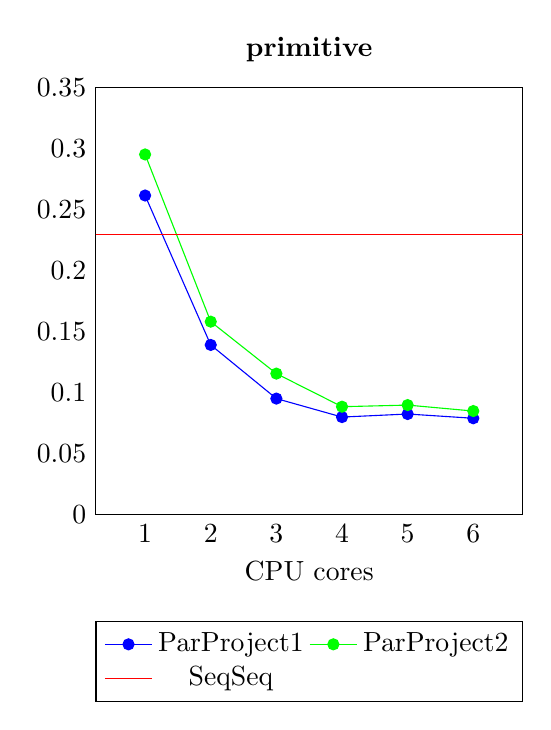
\begin{tikzpicture}
  \pgfplotsset{xtick style={draw=none}}
  \pgfplotsset{ytick style={draw=none}}
  \begin{axis}[
      width=7cm,
      height=7cm,
      enlargelimits=0.15,
      enlarge y limits=0,
      ymax=0.35,
      ymin=0,
      ytick distance=0.05,
      yticklabels={0,0,0.05,0.1,0.15,0.2,0.25,0.3,0.35},
      xtick=data,
      xlabel={CPU cores},
      xmin=1,
      xmax=6,
      xtick distance=1,
      title={\textbf{primitive}},
      legend style={
        at={(0.5,-0.25)},
        anchor=north,legend columns=2
      }
    ]
    \addplot[mark=*, blue] coordinates {
      (1,	0.26171)
      (2,	0.13912)
      (3,	0.09510)
      (4,	0.07994)
      (5,	0.08245)
      (6,	0.07896)
    };
    \addplot[mark=*, green] coordinates {
      (1,	0.29538)
      (2,	0.15821)
      (3,	0.11559)
      (4,	0.08845)
      (5,	0.08977)
      (6,	0.08489)
    };
    \addplot[mark=none, red] coordinates {
      (0,0.230)
      (7,0.230)
    };
    \legend{ParProject1, ParProject2, SeqSeq}
  \end{axis}
\end{tikzpicture}
~\hspace{-5pt}
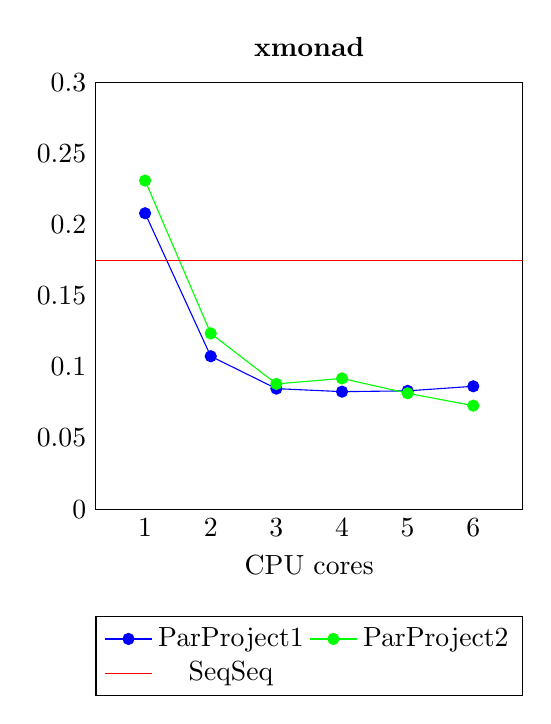
\begin{tikzpicture}
  \pgfplotsset{xtick style={draw=none}}
  \pgfplotsset{ytick style={draw=none}}
  \begin{axis}[
      width=7cm,
      height=7cm,
      enlargelimits=0.15,
      enlarge y limits=0,
      ymax=0.3,
      ymin=0,
      ytick distance=0.05,
      yticklabels={0,0,0.05,0.1,0.15,0.2,0.25,0.3},
      xtick=data,
      xlabel={CPU cores},
      xmin=1,
      xmax=6,
      xtick distance=1,
      title={\textbf{xmonad}},
      legend style={
        at={(0.5,-0.25)},
        anchor=north,legend columns=2
      }
    ]
    \addplot[mark=*, blue] coordinates {
      (1,	0.20805)
      (2,	0.10750)
      (3,	0.08473)
      (4,	0.08261)
      (5,	0.08317)
      (6,	0.08638)
    };
    \addplot[mark=*, green] coordinates {
      (1,	0.23102)
      (2,	0.12359)
      (3,	0.08807)
      (4,	0.09192)
      (5,	0.08147)
      (6,	0.07275)
    };
    \addplot[mark=none, red] coordinates {
      (0,0.175)
      (7,0.175)
    };
    \legend{ParProject1, ParProject2, SeqSeq}
  \end{axis}
\end{tikzpicture}
}\\

These results give us a couple of hints:

\begin{itemize}
\item If our \texttt{MTix} contains very few modules like the \textbf{bst} case
  study (only two modules), it is crucial to divide the inner sequences into
  chunks in order to use all the available CPUs.
\item When our \texttt{MTix} data contains a larger number of modules, the
  \textbf{ParProject2} variant carries a little overhead associated with the
  ``chunkification'' of the tasks. Otherwise they behave quite similarly.
\end{itemize}

With these considerations in mind, I would lean to use the \textbf{ParProject2}
variant, as I think it would give good results not only in large but also small
codebases.
%
Concretely, this variant achieves around 2x$\sim$3x of speedup.


\subsection*{Parallel Coverage}

For the last operation I consider in this report, I also implemented two
variants with different level of parallel granularity.

\paragraph{ParCoverage1}
Just like for the case of \textbf{ParProject1}, this first variant maps the
coverage operation over each module in parallel:

\begin{verbatim}
expCoverMTix :: [(String, Mix)] -> MTix -> [(String, Double)]
expCoverMTix mixs (MTix mods) = do
  parMap rdeepseq (expCoverMTixModule mixs) mods
\end{verbatim}

And as expected, we can see a (small) tail of uneven parallel work when we
inspect this computation using ThreadScope:\\

\includegraphics[scale=0.3]{threadscope/ParCoverage1}\\

To solve this issue, the next variant also reduces the parallel granularity of
the computation.

\paragraph{ParCoverage2}

As before, this implementation also splits the sequence of tick entries of each
module into chunks.
%
However, this computation also needs to combine the coverage results from each
chunk into a single one.
%
Thus, it is easy to see how this operation can be implemented in terms of a
parallel MapReduce combintator:

\begin{verbatim}
expCoverMTix :: [(String, Mix)] -> MTix -> [(String, Double)]
expCoverMTix mixs (MTix mods) = do
  parMap rdeepseq (expCoverMTixModule mixs) mods

expCoverMTixModule :: [(String, Mix)] -> MTixModule -> (String, Double)
expCoverMTixModule mixs (MTixModule name hash size tix) = do
  (name, (fromIntegral cov * 100) / fromIntegral tot)
  where
    (cov, tot) = mapReduceChunks rdeepseq 200 mapper reducer pairs
    reducer = foldr (\(c1, t1) (c2, t2) -> (c1+c2, t1+t2)) (0,0)
    mapper = foldr expCover (0,0)
    pairs = Seq.zip (Seq.fromList mix) tix
    Just (Mix _ _ _ _ mix)  = lookup (takeFileName name) mixs
    mixName (Mix m _ _ _ _) = takeFileName m
\end{verbatim}

\begin{verbatim}
mapReduceChunks :: Strategy b -> Int
                -> (Seq a -> b)
                -> (Seq b -> c)
                -> Seq a -> c
mapReduceChunks s n mapper reducer xs =
  reducer (fmap mapper chunks `using` parTraversable s)
  where
    chunks = Seq.chunksOf n xs
\end{verbatim}

After some manual tunning, I found that using chunks of 200 elements works
reasonably good on every case study.
%
If we inspect the ThreadScope output, we can see that the parallel work is now
more evenly distributed across cores:\\

\includegraphics[scale=0.3]{threadscope/ParCoverage2}\\

\paragraph{Benchmarks}

The final set of benchmarks presented in this report compare the performance of
the different expression coverage implementations:

% Parallel coverage
\resizebox{\textwidth}{!}{
\hspace{-50pt}
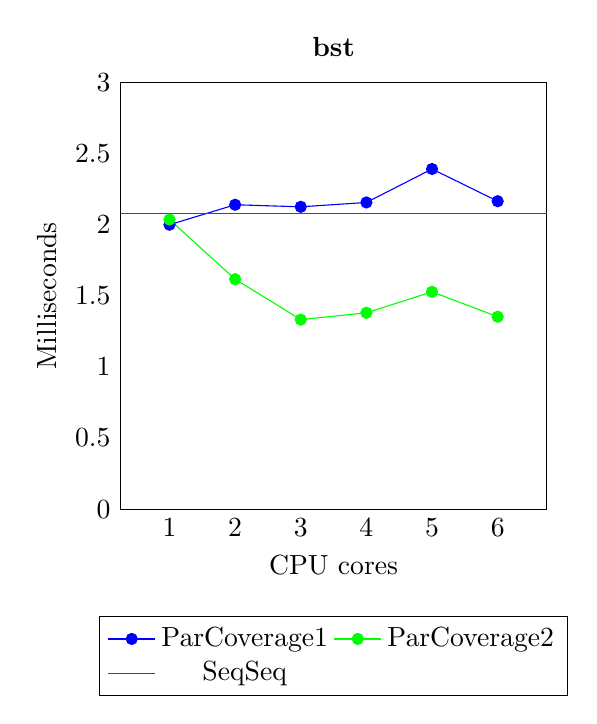
\begin{tikzpicture}
  \pgfplotsset{xtick style={draw=none}}
  \pgfplotsset{ytick style={draw=none}}
  \begin{axis}[
      width=7cm,
      height=7cm,
      enlargelimits=0.15,
      enlarge y limits=0,
      ymax=3,
      ymin=0,
      ytick distance=0.5,
      yticklabels={0,0,0.5,1,1.5,2,2.5,3},
      xtick=data,
      ylabel={Milliseconds},
      xlabel={CPU cores},
      xmin=1,
      xmax=6,
      xtick distance=1,
      title={\textbf{bst}},
      legend style={
        at={(0.5,-0.25)},
        anchor=north,legend columns=2
      }
    ]
    \addplot[mark=*, blue] coordinates {
      (1,	1.999798457)
      (2,	2.140306418)
      (3,	2.125807102)
      (4,	2.156469454)
      (5,	2.391723436)
      (6,	2.16521249)
    };
    \addplot[mark=*, green] coordinates {
      (1,	2.036091602)
      (2,	1.616879328)
      (3,	1.332552591)
      (4,	1.380659664)
      (5,	1.52799736)
      (6,	1.352924105)
    };
    \addplot[mark=none, red] coordinates {
      (0,2.076)
      (7,2.076)
    };
    \legend{ParCoverage1, ParCoverage2, SeqSeq}
  \end{axis}
\end{tikzpicture}
~\hspace{-5pt}
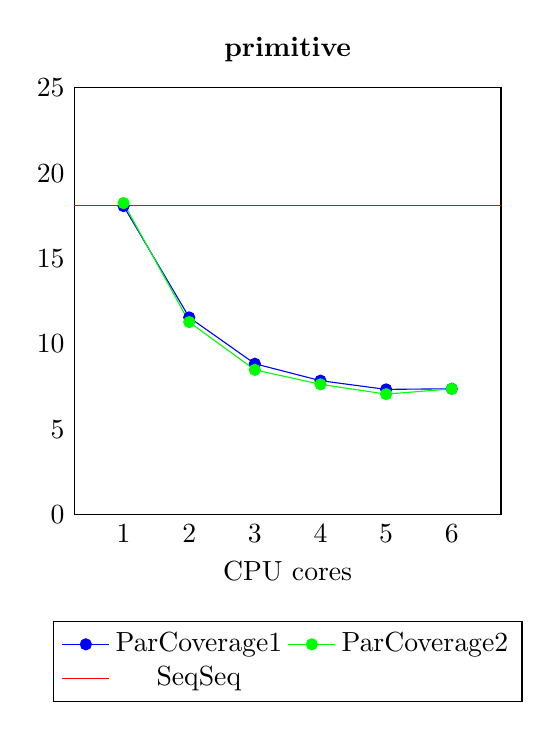
\begin{tikzpicture}
  \pgfplotsset{xtick style={draw=none}}
  \pgfplotsset{ytick style={draw=none}}
  \begin{axis}[
      width=7cm,
      height=7cm,
      enlargelimits=0.15,
      enlarge y limits=0,
      ymax=25,
      ymin=0,
      ytick distance=5,
      xtick=data,
      xlabel={CPU cores},
      xmin=1,
      xmax=6,
      xtick distance=1,
      title={\textbf{primitive}},
      legend style={
        at={(0.5,-0.25)},
        anchor=north,legend columns=2
      }
    ]
    \addplot[mark=*, blue] coordinates {
      (1,	18.07241404)
      (2,	11.54932487)
      (3,	8.835522228)
      (4,	7.843209439)
      (5,	7.331879587)
      (6,	7.369470515)
    };
    \addplot[mark=*, green] coordinates {
      (1,	18.24999386)
      (2,	11.27700625)
      (3,	8.477055719)
      (4,	7.628884595)
      (5,	7.054208489)
      (6,	7.363956561)
    };
    \addplot[mark=none, red] coordinates {
      (0,18.09)
      (7,18.09)
    };
    \legend{ParCoverage1, ParCoverage2, SeqSeq}
  \end{axis}
\end{tikzpicture}
~\hspace{-5pt}
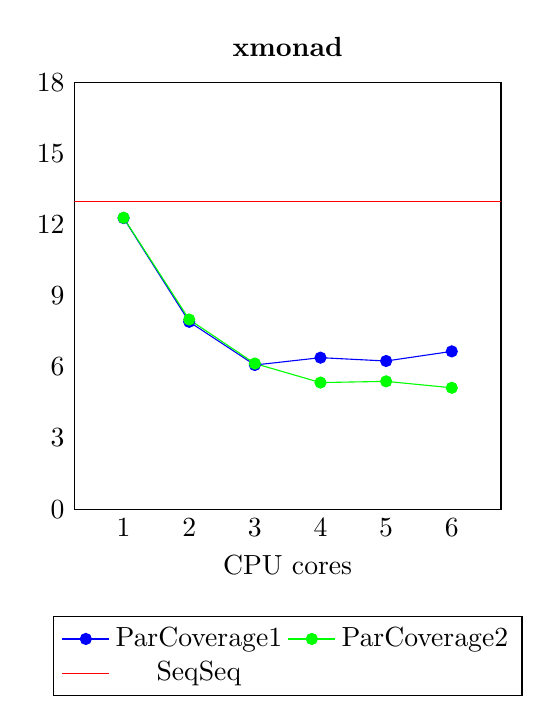
\begin{tikzpicture}
  \pgfplotsset{xtick style={draw=none}}
  \pgfplotsset{ytick style={draw=none}}
  \begin{axis}[
      width=7cm,
      height=7cm,
      enlargelimits=0.15,
      enlarge y limits=0,
      ymax=18,
      ymin=0,
      ytick distance=3,
      xtick=data,
      xlabel={CPU cores},
      xmin=1,
      xmax=6,
      xtick distance=1,
      title={\textbf{xmonad}},
      legend style={
        at={(0.5,-0.25)},
        anchor=north,legend columns=2
      }
    ]
    \addplot[mark=*, blue] coordinates {
      (1,	12.27925829)
      (2,	7.903431115)
      (3,	6.080712386)
      (4,	6.390404331)
      (5,	6.249881708)
      (6,	6.65609943)
    };
    \addplot[mark=*, green] coordinates {
      (1,	12.29389248)
      (2,	7.998992073)
      (3,	6.142958556)
      (4,	5.339186735)
      (5,	5.391108887)
      (6,	5.120059685)
    };
    \addplot[mark=none, red] coordinates {
      (0,12.98)
      (7,12.98)
    };
    \legend{ParCoverage1, ParCoverage2, SeqSeq}
  \end{axis}
\end{tikzpicture}
}\\

These results are similar to those obtained before for the projection operation,
except that here the most granular approach seems to outperform the less
granular one on every case study, and especially on the small \textbf{bst} one.
%
Concretely, \textbf{ParCoverage2} obtained speedups of between 1.5x to 2.5x.

\section*{Conclusions}

Altought in theory it seems rather easy, achieving a good level of parallelism
in Haskell can be quite intricate, as it requires a large variety of case
studies to test with, and a good eye for finding the best parallel granularity.

Some operations like map and map-reduce are relatively straightforward to
implement and to tweak.
%
However, others like transpositions of data, e.g., the merge operation here, are
more tricky to reason about, especially if we consider Haskell's lazy
evaluation, and the contradicting fact that we are sometimes forced to fully
evaluate things in order to get better parallelism.

However, even if I only managed to obtain a $\sim$0.75x speedup per core the
best scenario I tested (and almost none in the worst), the results I found
throughout this project motivate me to continue digging on the future ideas
behind it, namely test-suite reduction and better dynamic coverage reports.


%%%%%%%%%%%%%%%%%%%%%%%%%%%%%%%%%%%%%%%%
% Bibliography

\begin{thebibliography}{}
  \bibitem{hpc}
    Gill, Andy, and Colin Runciman. "Haskell program coverage."
    Proceedings of the ACM SIGPLAN Workshop on Haskell. 2007.
  \bibitem{tasty-quickcheck-hpc}
    \url{https://github.com/agustinmista/tasty-quickcheck-hpc}
  \bibitem{hpcpp}
    \url{https://github.com/agustinmista/hpcpp}
  \bibitem{primitive}
    \url{http://hackage.haskell.org/package/primitive}
  \bibitem{xmonad}
    \url{http://hackage.haskell.org/package/xmonad}
  \bibitem{data-map}
    \url{https://hackage.haskell.org/package/containers-0.6.2.1/docs/Data-Map-Strict.html}
  \bibitem{data-sequence}
    \url{https://hackage.haskell.org/package/containers-0.6.3.1/docs/Data-Sequence.html}
  \bibitem{seq-no-more}
    Marlow, S., Maier, P., Loidl, H. W., Aswad, M. K., and Trinder, P. (2010).
    Seq no more: better strategies for parallel Haskell. ACM Sigplan Notices,
    45(11), 91-102.
\end{thebibliography}

\end{document}
